\documentclass[12pt,a4paper]{article}
\usepackage[UTF8]{ctex}
\usepackage{amsmath,amssymb}
\usepackage{listings}
\usepackage{xcolor}
\usepackage{hyperref}
\usepackage{geometry}
\usepackage{graphicx}
\geometry{margin=2.5cm}

\lstdefinestyle{python}{
  language=Python,
  basicstyle=\ttfamily\small,
  keywordstyle=\color{blue}\bfseries,
  commentstyle=\color{gray},
  stringstyle=\color{red},
  showstringspaces=false,
  breaklines=true,
  frame=single,
  backgroundcolor=\color{gray!10}
}

\title{Shor Code / Shor 码}
\author{QuoNic}
\date{}

\begin{document}
\maketitle

\begin{center}
\textbf{Error Correction / 纠错} | 难度：高级 | 预计时间：20 分钟
\end{center}

\tableofcontents
\newpage

\section{为什么需要？}

Shor 码是第一个完整的量子纠错码，可以同时纠正比特翻转和相位翻转错误。

\subsection{经典局限}
\begin{itemize}
  \item 比特翻转码只能纠正 $X$ 错误
  \item 相位翻转码只能纠正 $Z$ 错误
  \item 实际量子系统同时存在两种错误
\end{itemize}

\subsection{量子优势}
\begin{itemize}
  \item Shor 码用 9 个物理量子比特编码 1 个逻辑量子比特
  \item 可以纠正任意单量子比特错误
  \item 是量子纠错的里程碑
\end{itemize}

\subsection{实际应用}
\begin{itemize}
  \item 量子计算（通用纠错）
  \item 量子通信（保护量子态）
  \item 量子存储（延长相干时间）
\end{itemize}

\section{快速上手}

\begin{lstlisting}[style=python]
from quonic.qec import shor_code

# Encode, introduce error, correct
result = shor_code(error_type="X", error_qubit=0)
print(f"Original: {result.original}")
print(f"Corrected: {result.corrected}")
\end{lstlisting}

\textbf{预期输出}：
\begin{verbatim}
Original: |0>
Corrected: |0>
\end{verbatim}

\section{原理详解}

\subsection{电路图}

\begin{center}
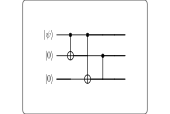
\includegraphics[width=0.7\textwidth]{../../images/shor_code_circuit.svg}
\end{center}

\subsection{数学推导}

Shor 码将 1 个逻辑量子比特编码到 9 个物理量子比特：
\begin{equation}
|0\rangle_L = \frac{1}{2\sqrt{2}}(|000\rangle + |111\rangle)^{\otimes 3}
\end{equation}
\begin{equation}
|1\rangle_L = \frac{1}{2\sqrt{2}}(|000\rangle - |111\rangle)^{\otimes 3}
\end{equation}

\textbf{编码过程}：
\begin{enumerate}
  \item 先用相位翻转码编码（3 个块）
  \item 再用比特翻转码编码每个块
\end{enumerate}

\textbf{纠错过程}：
\begin{enumerate}
  \item 检测每个块内的比特翻转错误
  \item 检测块间的相位翻转错误
  \item 纠正检测到的错误
\end{enumerate}

\subsection{几何解释}

Shor 码通过级联编码，将相位翻转码和比特翻转码组合，实现通用纠错。

\section{代码详解}

\begin{lstlisting}[style=python]
from quonic.qec import shor_code

# shor_code(error_type, error_qubit)
# error_type: "X", "Z", or "Y"
# error_qubit: which qubit has the error
result = shor_code(error_type="X", error_qubit=0)

# result.original: original state
# result.encoded: encoded state
# result.error: state after error
# result.corrected: corrected state
print(f"Corrected: {result.corrected}")
\end{lstlisting}

\section{进阶用法}

\subsection{场景 1：不同错误类型}

\begin{lstlisting}[style=python]
# Different error types
for error_type in ["X", "Z", "Y"]:
    result = shor_code(error_type=error_type, error_qubit=0)
    print(f"{error_type} error: {result.corrected}")
\end{lstlisting}

\subsection{场景 2：不同错误位置}

\begin{lstlisting}[style=python]
# Error on different qubits
for i in range(9):
    result = shor_code(error_type="X", error_qubit=i)
    print(f"Error on q{i}: {result.corrected}")
\end{lstlisting}

\section{适用场景}

\subsection{量子计算}

Shor 码是量子计算的基础纠错码。

\subsection{量子通信}

Shor 码可以保护量子通信中的量子态。

\subsection{量子存储}

Shor 码可以延长量子存储的相干时间。

\section{常见问题}

\subsection{Shor 码需要多少量子比特？}

需要 9 个物理量子比特编码 1 个逻辑量子比特。

\subsection{Shor 码能纠正所有错误吗？}

Shor 码可以纠正任意单量子比特错误，但不能纠正多量子比特错误。

\subsection{Shor 码和表面码有什么区别？}

Shor 码是级联码，表面码是拓扑码。表面码有更好的容错阈值。

\section{学习路径}

\subsection{前置知识}
\begin{itemize}
  \item 比特翻转码
  \item 相位翻转码
  \item 量子测量
\end{itemize}

\subsection{继续学习}
\begin{itemize}
  \item Steane 码
  \item 表面码
  \item 颜色码
\end{itemize}

\section{完整示例代码}

\subsection{示例 1：基本 Shor 码}

\begin{lstlisting}[style=python]
from quonic.qec import shor_code

result = shor_code(error_type="X", error_qubit=0)
print(f"Corrected: {result.corrected}")
\end{lstlisting}

\end{document}
